\documentclass[aspectratio=169, 14pt]{beamer}
\usepackage[utf8]{inputenc}
\usepackage[english]{babel}
\usepackage{tipa}
\usepackage{graphicx}
\usepackage{transparent}
\usepackage[ruled, lined, linesnumbered, commentsnumbered]{algorithm2e}
\usepackage{pgfplots}
\usepackage{tikz}
\usetikzlibrary{calc,shadows.blur}
\usetikzlibrary{matrix,backgrounds}
\usetikzlibrary{arrows, positioning}
\usetikzlibrary {arrows.meta}
\usetikzlibrary{decorations.pathmorphing, patterns}
\pgfdeclaredecoration{penciline}{initial}{
	\state{initial}[width=+\pgfdecoratedinputsegmentremainingdistance,auto corner on length=1mm,]{
		\pgfpathcurveto%
		{% From
			\pgfqpoint{\pgfdecoratedinputsegmentremainingdistance}
			{\pgfdecorationsegmentamplitude}
		}
		{%  Control 1
			\pgfmathrand
			\pgfpointadd{\pgfqpoint{\pgfdecoratedinputsegmentremainingdistance}{0pt}}
			{\pgfqpoint{-\pgfdecorationsegmentaspect\pgfdecoratedinputsegmentremainingdistance}%
				{\pgfmathresult\pgfdecorationsegmentamplitude}
			}
		}
		{%TO 
			\pgfpointadd{\pgfpointdecoratedinputsegmentlast}{\pgfpoint{1pt}{1pt}}
		}
	}
	\state{final}{}
}
\usepackage{minted}
\usepackage{fontawesome5}
\usepackage{booktabs}
\usepackage{hyperref}
\hypersetup{
	colorlinks=true,
	linkcolor=blue,
	filecolor=magenta,
	urlcolor=cyan,
}
\urlstyle{same}
\usetheme{metropolis}
\metroset{block=fill}
\usecolortheme{default}
\definecolor{darkmidnightblue}{rgb}{0.0, 0.2, 0.4}
\definecolor{LightGray}{gray}{0.9}


%------------------------------------------------------------
%This block of code defines the information to appear in the
%Title page
\title[Data Structures] %optional
{Data Structures}

\subtitle{Stacks}

\author[CHEN Zhongpu] % (optional)
{CHEN Zhongpu}

\institute[] % (optional)
{
	School of Computing and Artificial Intelligence \\
	\href{mailto:zpchen@swufe.edu.cn}{zpchen@swufe.edu.cn}
}

\date[] % (optional)
{SWUFE, Fall \the\year{}}

%End of title page configuration block
%------------------------------------------------------------


%------------------------------------------------------------
%The next block of commands puts the table of contents at the 
%beginning of each section and highlights the current section:

% \AtBeginSection[]
% {
%   \begin{frame}
%     \frametitle{Table of Contents}
%     \tableofcontents[currentsection]
%   \end{frame}
% }
%------------------------------------------------------------


\begin{document}

%The next statement creates the title page.
\frame{\titlepage}

%---------------------------------------------------------
%This block of code is for the table of contents after
%the title page
% \begin{frame}
% \frametitle{Table of Contents}
% \tableofcontents
% \end{frame}
%--------------------------------------------------------
\begin{frame}[fragile]
	\frametitle{A Small Quiz}

	What is time complexity of the following code in the worst-case?
	\begin{minted}[bgcolor=LightGray, fontsize=\small]{python}
def find_max(a):
    m = a[0]
    for i in a:
        if i > m:
            m = i
    return m

def find_max2(a):
    return max(a)
\end{minted}

\end{frame}


{
% \usebackgroundtemplate{\transparent{0.3}{\begin{picture}
%     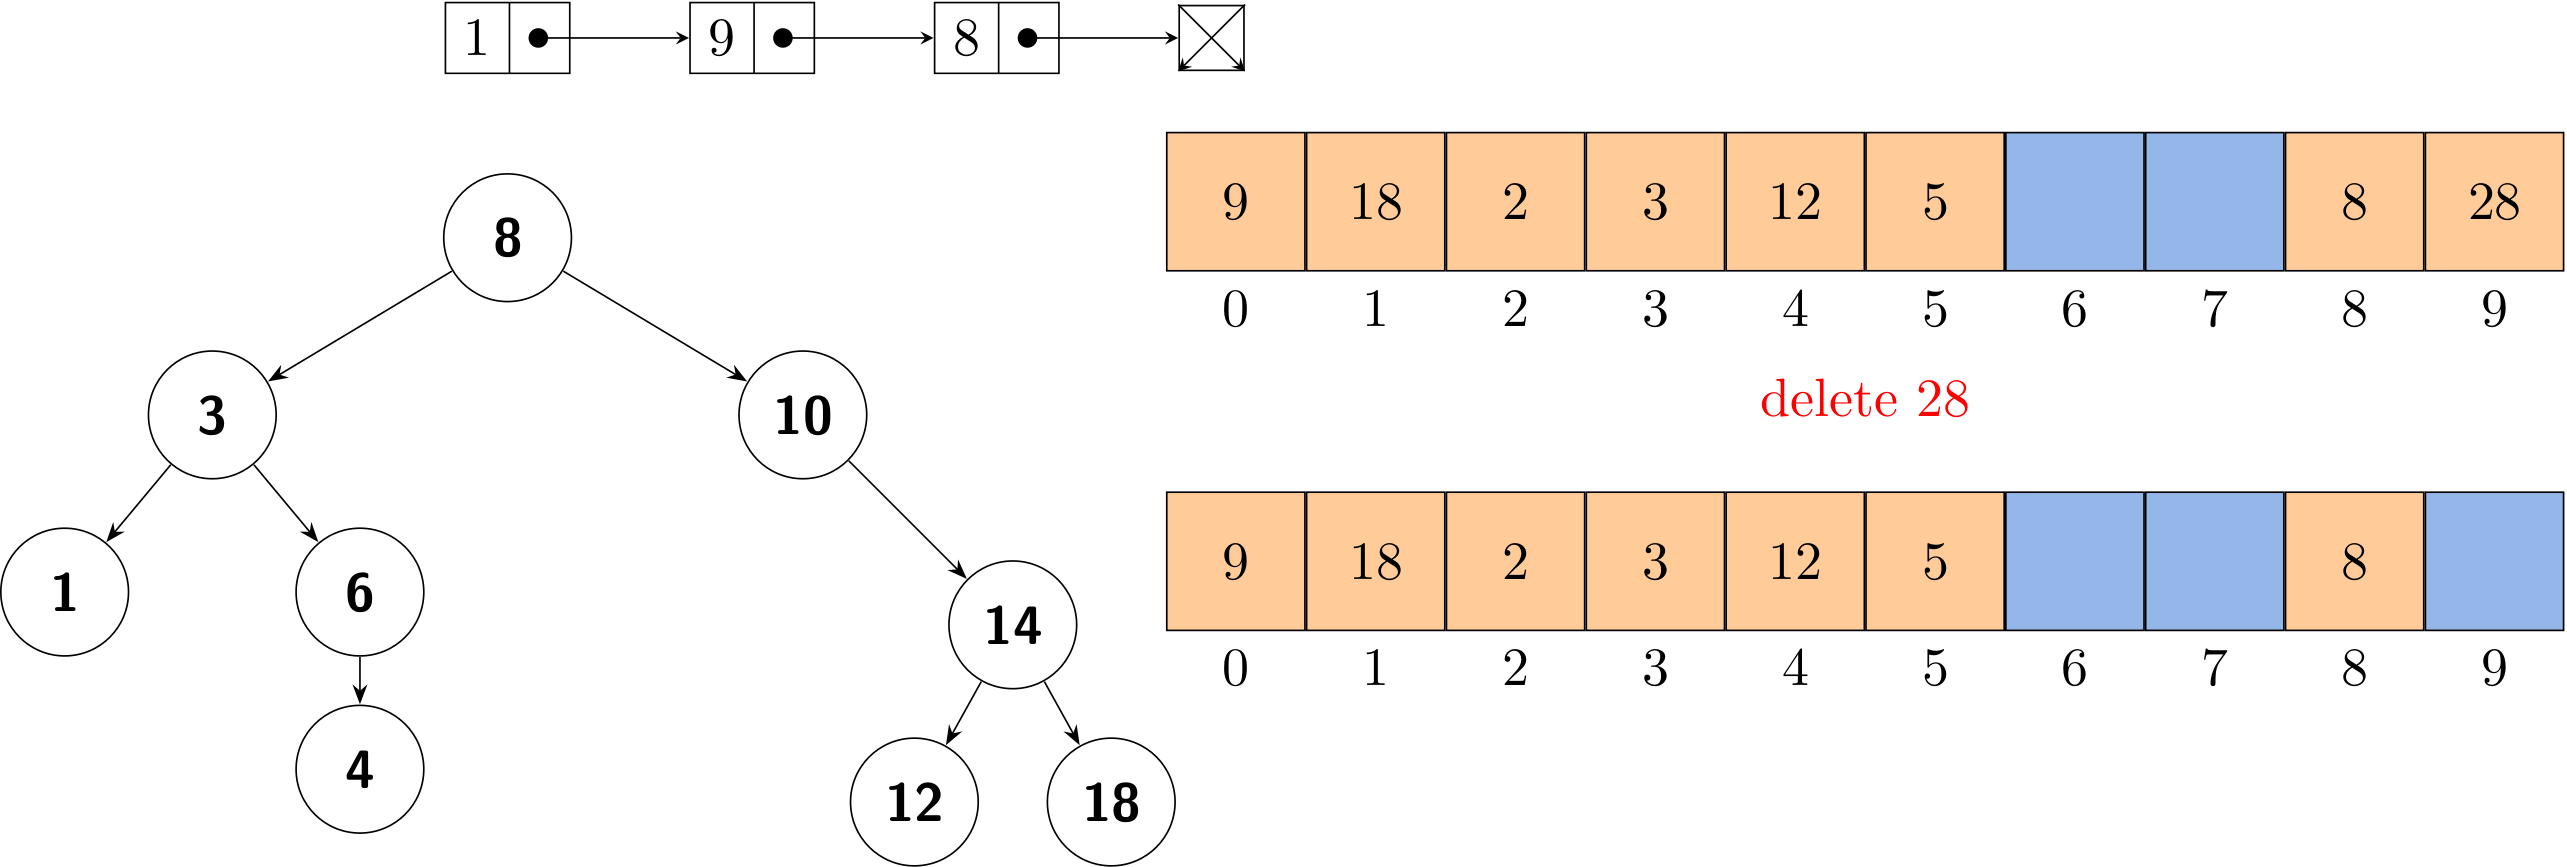
\includegraphics[height=0.7\paperheight]{cover}
% \end{picture}    
% }}
\usebackgroundtemplate{
	\tikz[overlay,remember picture]
	\node[opacity=0.3, at=(current page.south east),anchor=south east, yshift=2cm,xshift=4cm] {
		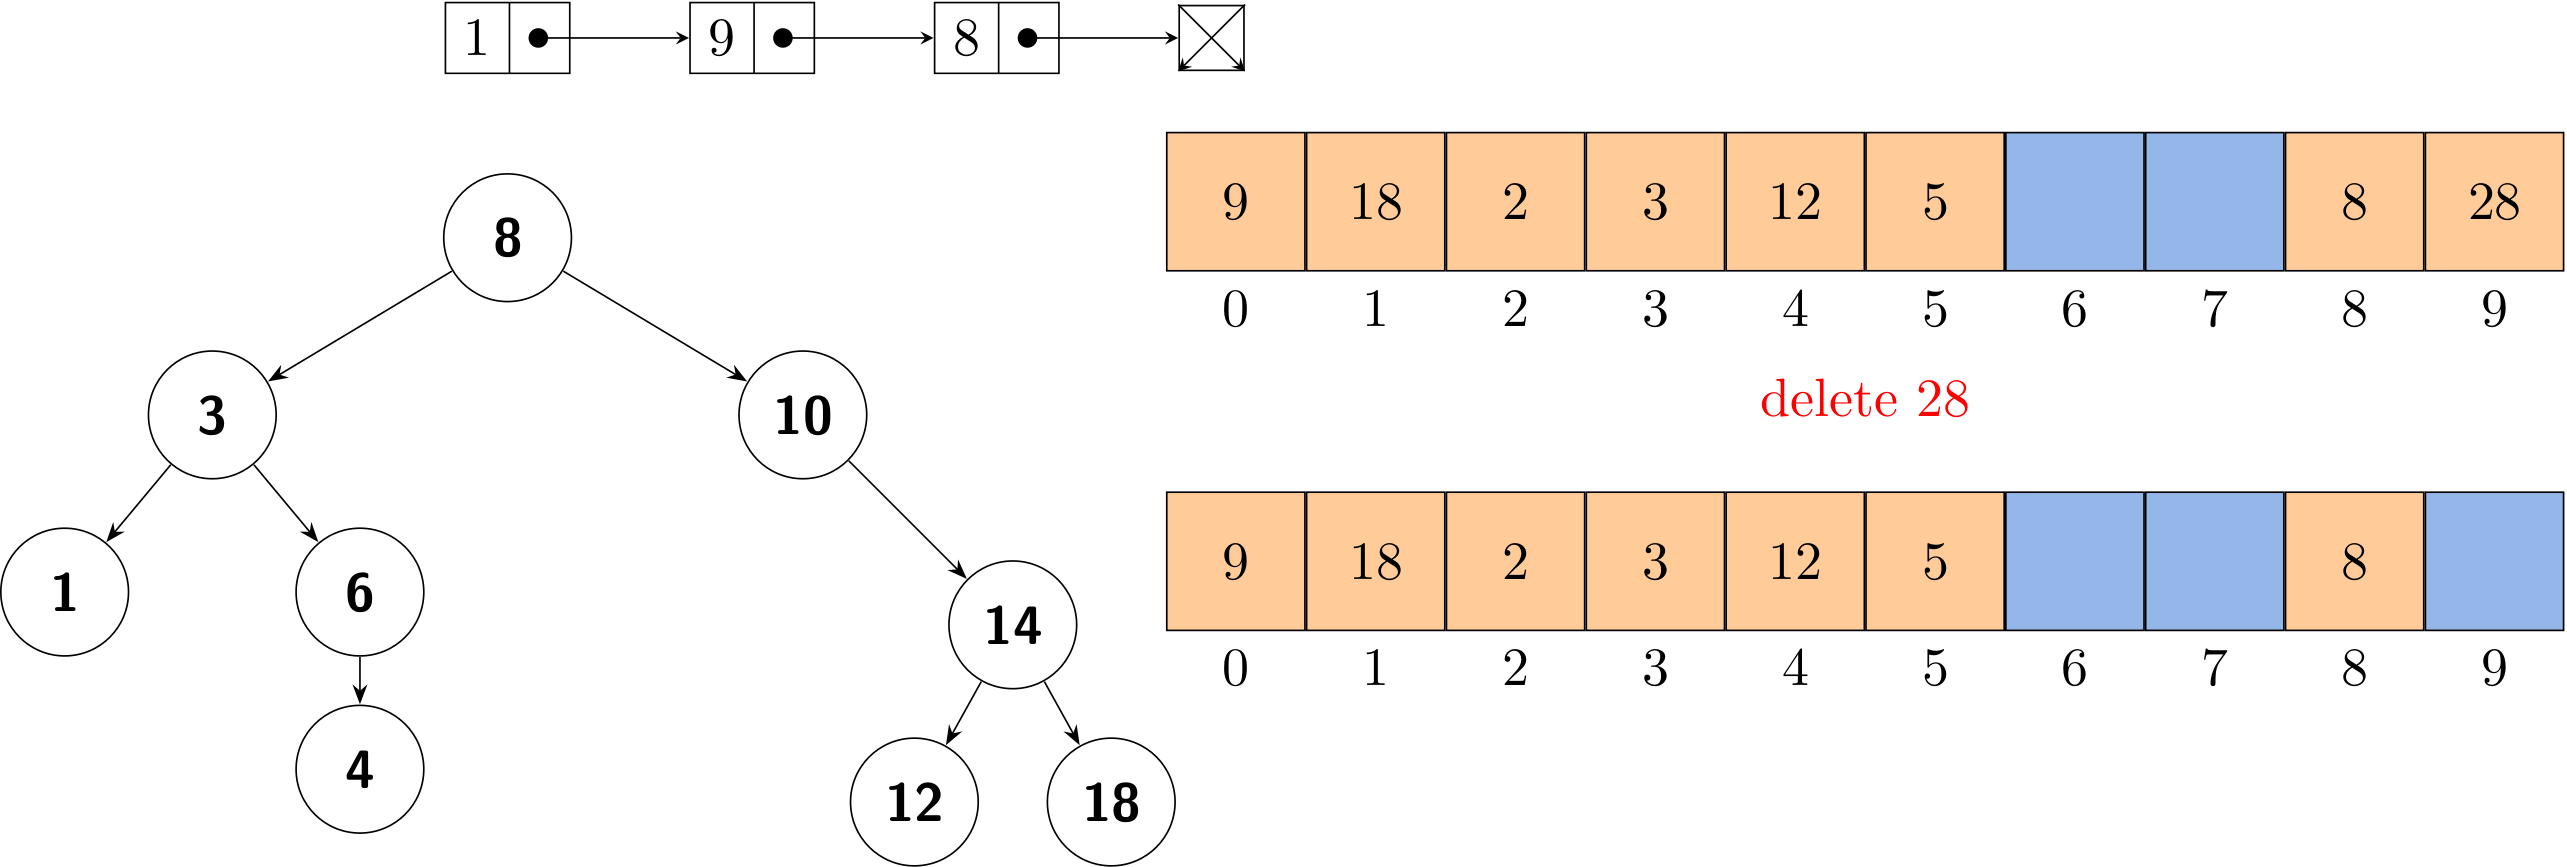
\includegraphics[height=0.6\paperheight]{cover}};
}
\begin{frame}
	\section{\textcolor{darkmidnightblue}{ADT}}
\end{frame}
}

\begin{frame}[fragile]
	\frametitle{Revisit}
	We have implemented a self-defined \alert{Array}.

	\begin{minted}[bgcolor=LightGray]{python}
arr = Array(5)
print(len(arr))
arr[4] = 7
print(arr[4])
for i in arr:
  print(i)
\end{minted}

	To use \alert{Array}, do we need to know how it is implemented?
\end{frame}

\begin{frame}
	\frametitle{ADT}
	\begin{exampleblock}{ADT}
		An abstract data type (ADT) is a data type whose representation is hidden from the client.
	\end{exampleblock}
	\begin{itemize}
		\item To use an ADT, we mainly focus on the operations specified in its \alert{API}.
		\item To implement an ADT, we focus on the data, then implement operations on that data.
	\end{itemize}
\end{frame}
{
% \usebackgroundtemplate{\transparent{0.3}{\begin{picture}
%     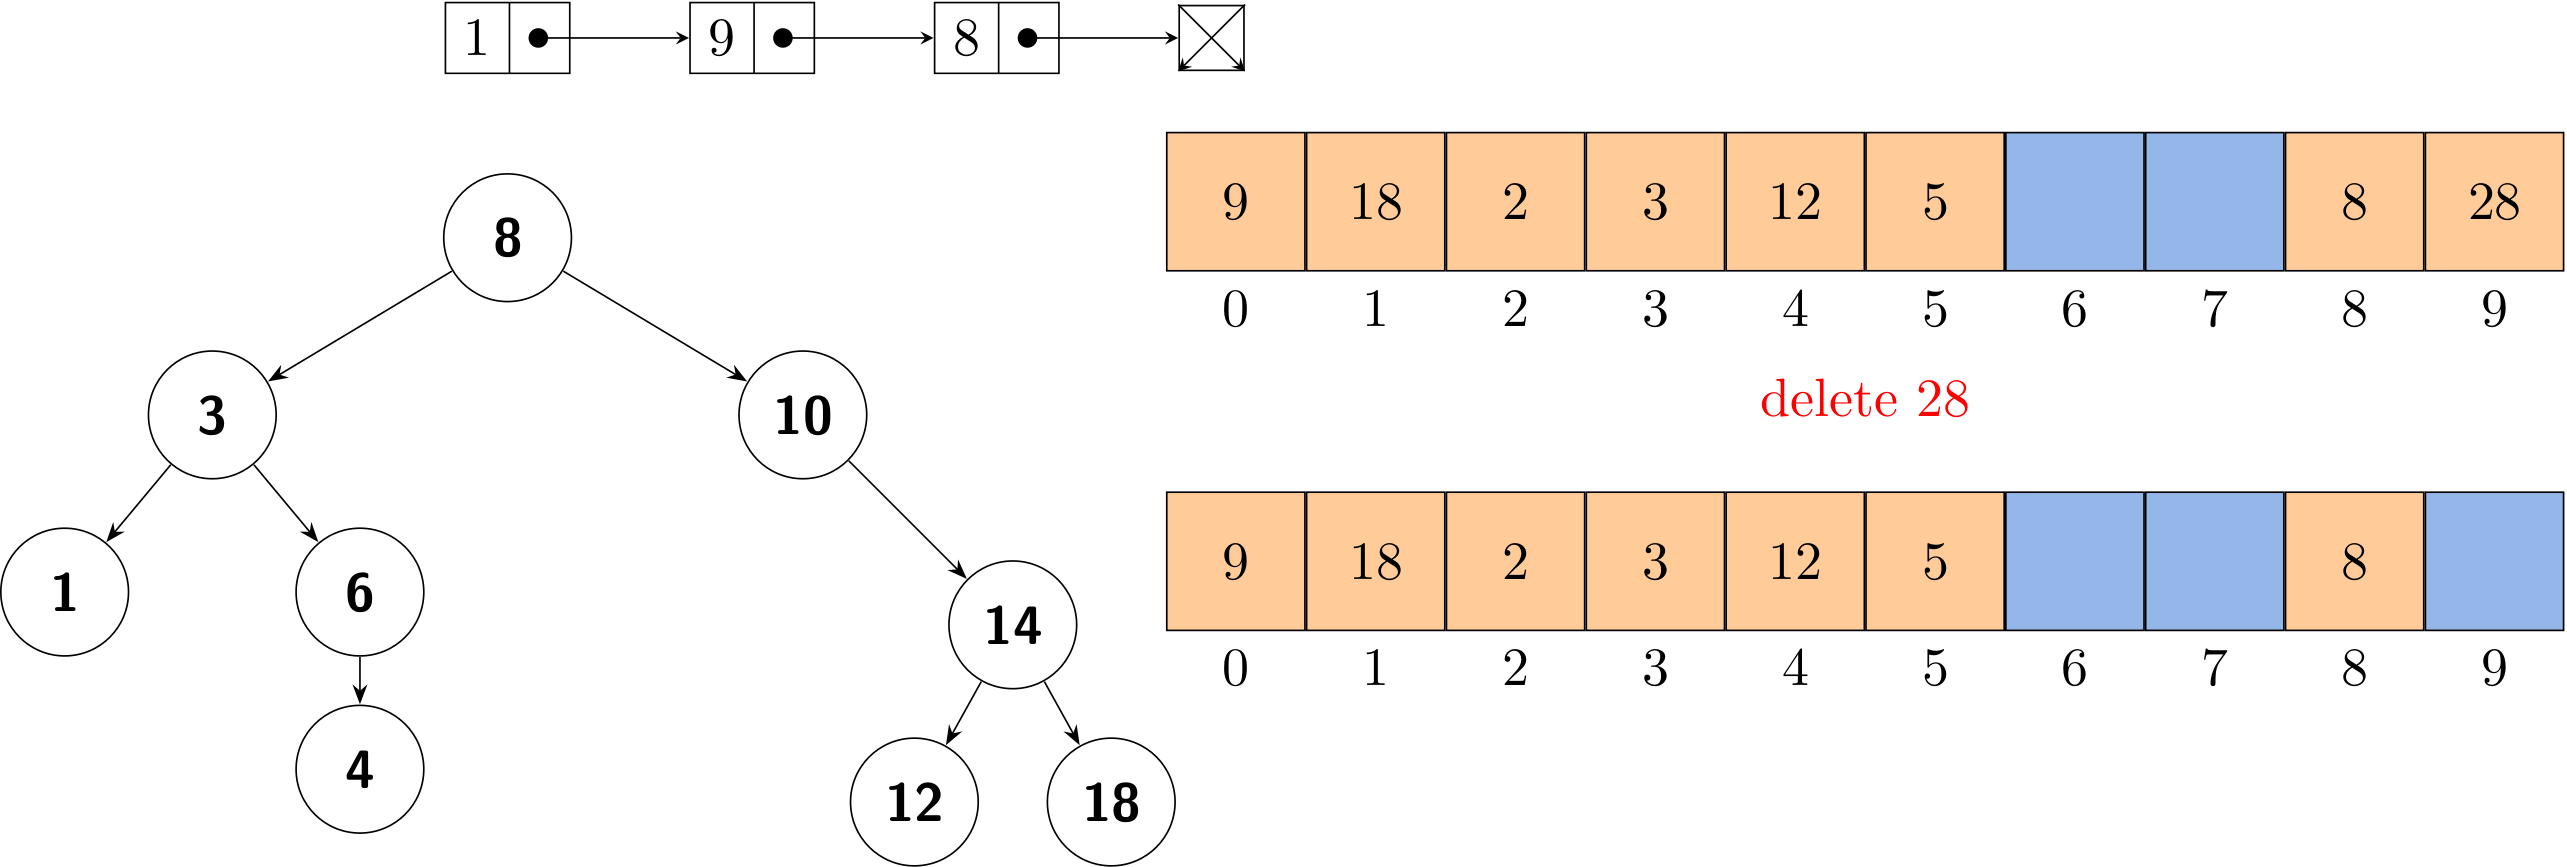
\includegraphics[height=0.7\paperheight]{cover}
% \end{picture}    
% }}
\usebackgroundtemplate{
	\tikz[overlay,remember picture]
	\node[opacity=0.3, at=(current page.south east),anchor=south east, yshift=2cm,xshift=4cm] {
		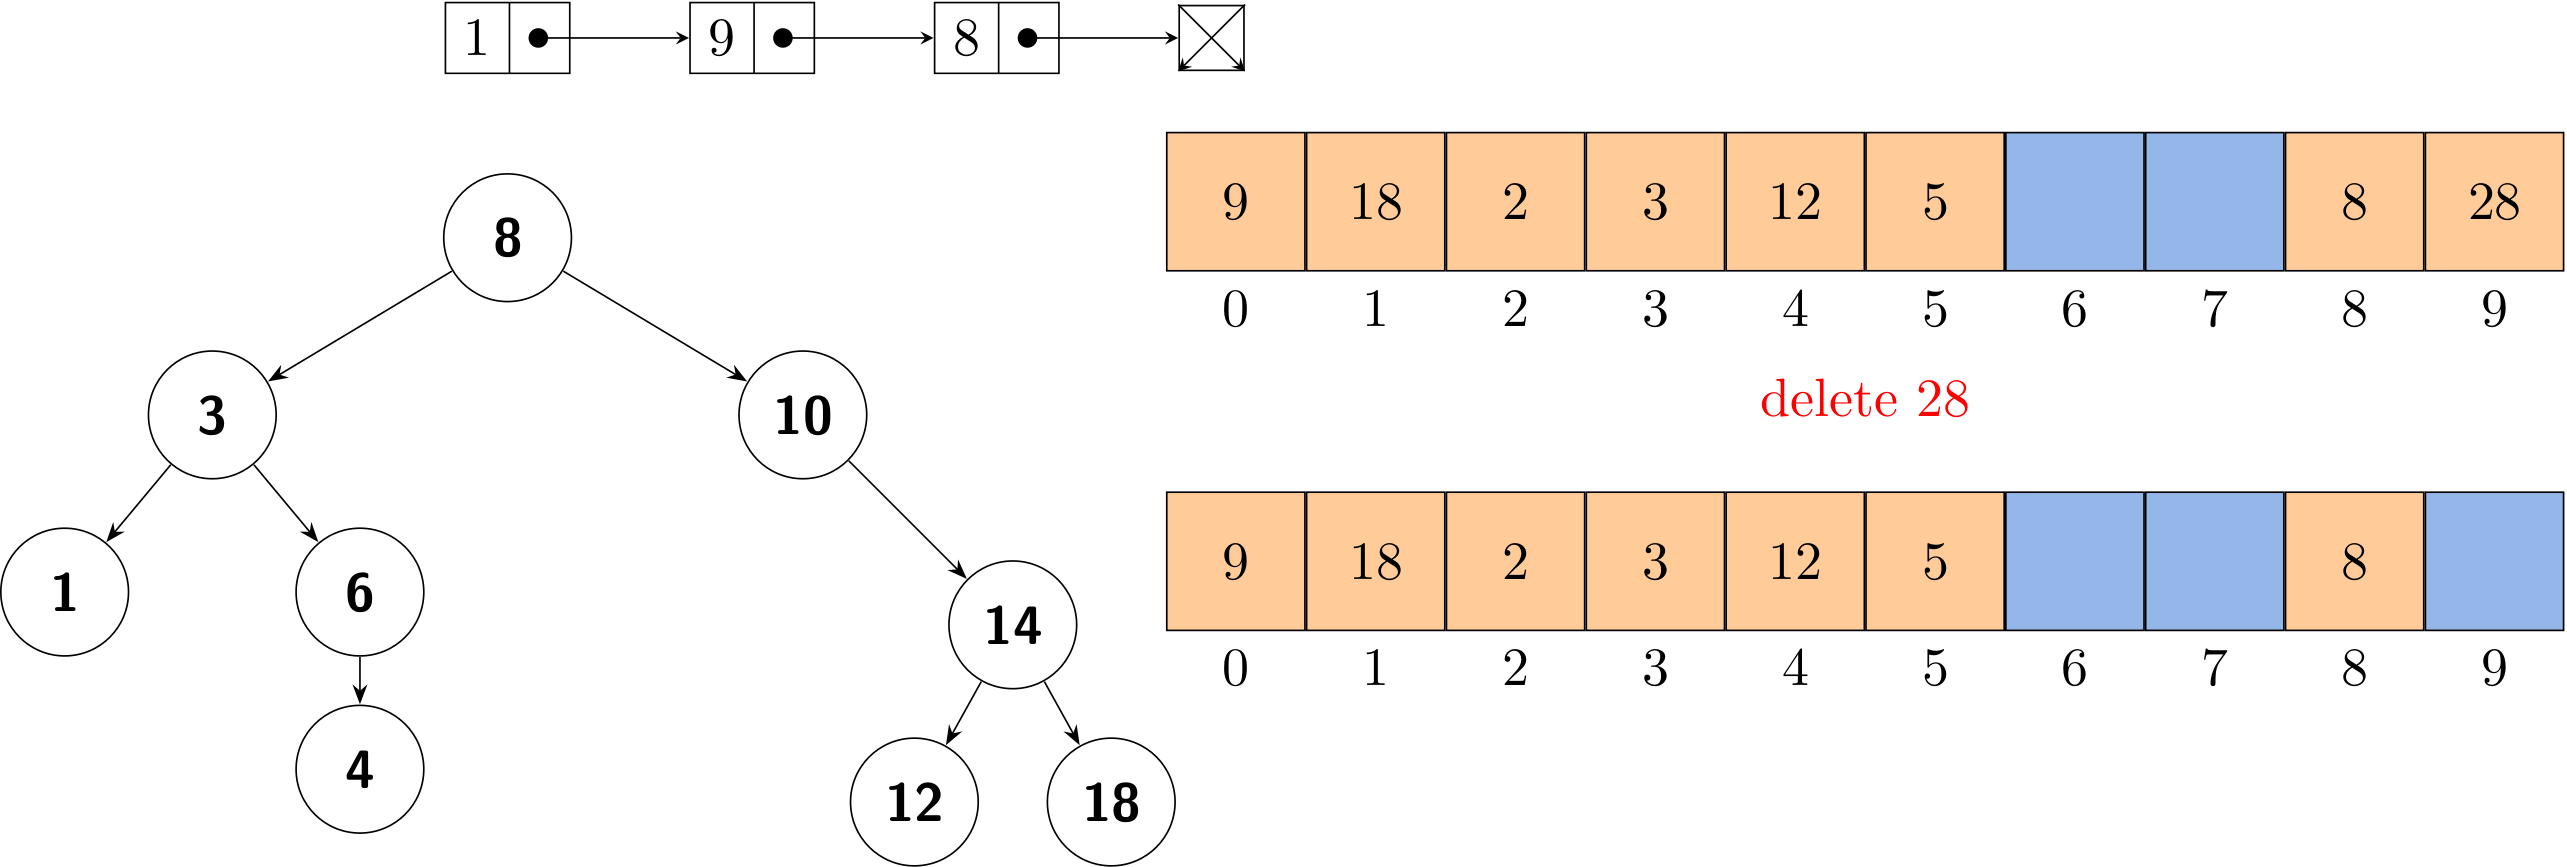
\includegraphics[height=0.6\paperheight]{cover}};
}
\begin{frame}
	\section{\textcolor{darkmidnightblue}{1. Stacks}}
\end{frame}
}

\begin{frame}[fragile]
	\frametitle{Example: Web Pages}

	\begin{columns}
		\column{0.5\textwidth}
		\begin{verbatim}
<!-- a.html -->
<a href="b.html">Next</a>

<!-- b.html -->
<a href="c.html">Next</a>

<!-- c.html -->
<a href="d.html">Next</a>
        \end{verbatim}
		\column{0.5\textwidth}
		Suppose you are visiting \textbf{a.html}, and then click "Next". Continue to click "Next" until reaching \textbf{d.html}. Now start to consider click "Back".
	\end{columns}

\end{frame}

\begin{frame}
	\begin{quote}
		Stack: a pile of things arranged one on top of another.
		\begin{flushright}
			--- From Cambridge Dictionary
		\end{flushright}
	\end{quote}
	\begin{figure}
		
\includegraphics[width=0.4\textwidth, height=0.4\paperheight]{week3/book}
		\hfill
		
\includegraphics[width=0.4\textwidth, height=0.4\paperheight]{week3/tray}
	\end{figure}

	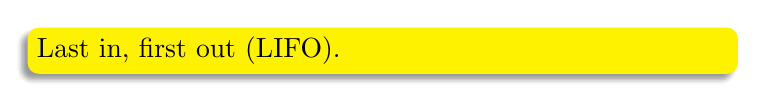
\begin{tikzpicture}
		\node[fill=yellow,blur shadow={shadow xshift=-0.5ex},
			text width=25em,anchor=south west,rounded corners]
		{Last in, first out (LIFO).
		};
	\end{tikzpicture}
\end{frame}

\begin{frame}
	\frametitle{1.1 Stack}
	\begin{exampleblock}{Stack}
		A stack is a collection of objects that are inserted and removed according to the \alert{last-in, first-out (LIFO)} policy.
	\end{exampleblock}
	It supports two basic operations:
	\begin{itemize}
		\item \texttt{push()}: add a new element
		\item \texttt{pop()}: remove an element
	\end{itemize}
	Additionally, it also supports other operations such as \texttt{size()}, \texttt{isEmpty()}, and \texttt{top()}.
\end{frame}

\begin{frame}[fragile]
	\frametitle{Stack in Python}
	Fortunately, the \texttt{list} in Python supports the operations required by stacks.
	\begin{minted}[bgcolor=LightGray]{python}
s = []
s.append('a') # append() works like push()
s.append('b')
s.append('c')
print(len(s))
print(s.pop())
print(s.pop())
print(len(s))
\end{minted}

\end{frame}

\begin{frame}[fragile]
	Let's implement our own \alert{Stack} in the object-oriented way.
	\begin{minted}[bgcolor=LightGray, fontsize=\small]{python}
s = Stack()
s.push('a')
s.push('b')
s.push('c')
print(s.size())
print(s.pop())
print(s.pop())
print(s.size())
\end{minted}

\end{frame}

\begin{frame}[fragile]
	We use \alert{list} as the underlying data structure.
	\begin{minted}[fontsize=\small,bgcolor=LightGray]{python}
class Stack:
    def __init__(self):
        self._data = []
    def push(self, item):
        pass
    def pop(self):
        pass
    def size(self):
        pass
    def is_empty(self):
        pass
\end{minted}

\end{frame}

\begin{frame}[fragile]
	\begin{minted}[bgcolor=LightGray]{python}
def push(self, item):
    self._data.append(item)    
\end{minted}

	\begin{minted}[bgcolor=LightGray]{python}
def pop(self):
    return self._data.pop()   
\end{minted}

	\begin{minted}[bgcolor=LightGray]{python}
def size(self):
    return len(self._data)    
    \end{minted}
\end{frame}

\begin{frame}[fragile]
	\frametitle{Exception}
	\begin{block}{Exception}
		You need also consider the condition that cannot be handled by the "normal flow".
	\end{block}

	{\large \faIcon{question-circle}} What will happen if we \texttt{pop} from an empty stack?
	\begin{minted}[bgcolor=LightGray, fontsize=\small]{python}
s = Stack()
print(s.pop())
\end{minted}

\end{frame}

\begin{frame}[fragile]
	But we would like a self-defined exception (error) for stack ADT.

	\begin{minted}[fontsize=\small,bgcolor=LightGray, breaklines=true]{python}
class NoElement(Exception):
    """Error attempting to access an element from an empty collection."""
    pass
def pop(self):
    if self.is_empty():
        raise NoElement('Pop from empty stack!')
    return self._data.pop()  
\end{minted}
\end{frame}

\begin{frame}[fragile]
	Yet another philosophy to handle exception in addition to \alert{look-before-you-leap}.

	\begin{minted}[fontsize=\small,bgcolor=LightGray, breaklines=true]{python}
def pop(self):
  try:
    return self._data.pop()
  except:
    raise NoElement('Pop from empty stack!')
\end{minted}
\end{frame}

\begin{frame}
	\frametitle{1.2 Time complexity}
	\begin{table}
		\caption{Stack's time complexity}
		\begin{tabular}{lr}
			\toprule
			Operation            & Complexity \\
			\midrule
			\texttt{push()}      & $O(1)$     \\
			\texttt{pop()}       & $O(1)$     \\
			\texttt{size()}      & $O(1)$     \\
			\texttt{is\_empty()} & $O(1)$     \\
			\bottomrule
		\end{tabular}
	\end{table}

	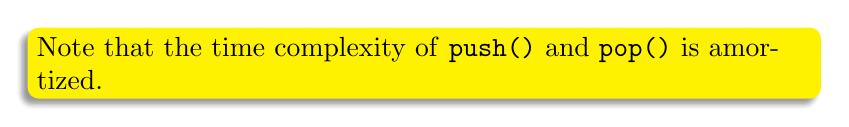
\begin{tikzpicture}
		\node[fill=yellow,blur shadow={shadow xshift=-0.5ex},
			text width=28em,anchor=south west,rounded corners]
		{Note that the time complexity of \texttt{push()} and \texttt{pop()} is amortized.
		};
	\end{tikzpicture}
\end{frame}

\begin{frame}[fragile]
	\frametitle{1.3 Resizing}
	Basically, an amortized time is \textbf{the average time taken per operation, if you do many operations}.

	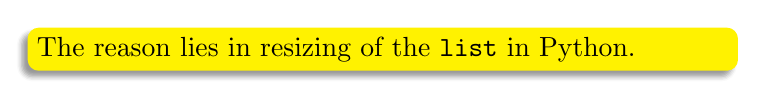
\begin{tikzpicture}
		\node[fill=yellow,blur shadow={shadow xshift=-0.5ex},
			text width=25em,anchor=south west,rounded corners]
		{The reason lies in \alert{resizing} of the \texttt{list} in Python.
		};
	\end{tikzpicture}
	\pause
	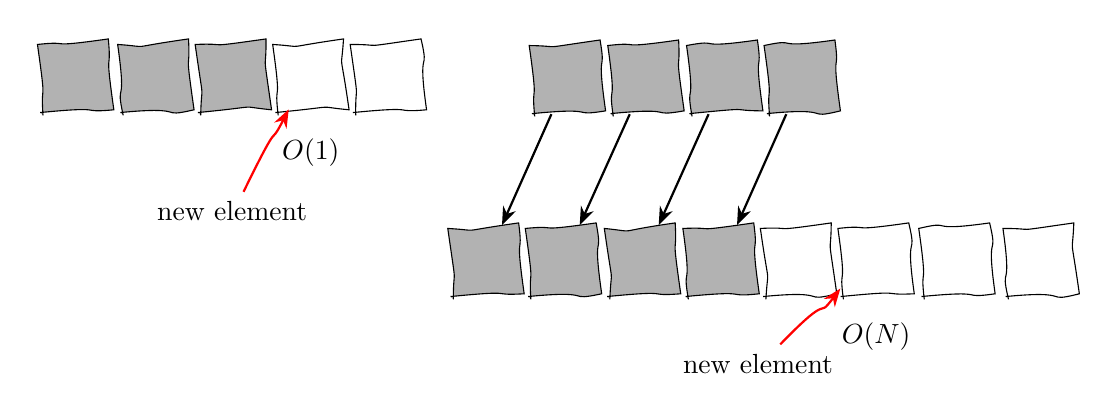
\begin{tikzpicture}[slot/.style={minimum size=0.9cm,rectangle}, data/.style={slot, fill=black!30}, >=Stealth, decoration=penciline]
		\matrix [nodes=draw] (table1)
		{
			\node[data, decorate] {};          &
			\node[data, decorate] {};          &
			\node[data, decorate] {};          &
			\node[slot, decorate] (insert) {}; &
			\node[slot, decorate] {};
			\\
		};
		\node[below=of insert, xshift=-1cm] (start) {new element};
		\draw[->,thick,red, decorate] (start) -- (insert);
		\node[below=of insert, yshift=0.8cm] {$O(1)$};

		\matrix [nodes=draw, right=of table1](table2)
		{
			\node[data, decorate] (2n1) {}; &
			\node[data, decorate] (2n2) {}; &
			\node[data, decorate] (2n3) {}; &
			\node[data, decorate] (2n4) {};
			\\
		};

		\matrix [nodes=draw, below=of table2, xshift=1cm](table3)
		{
			\node[data, decorate] (3n1) {};     &
			\node[data, decorate] (3n2) {};     &
			\node[data, decorate] (3n3) {};     &
			\node[data, decorate] (3n4) {};     &
			\node[slot, decorate] {};           &
			\node[slot, decorate] (insert2) {}; &
			\node[slot, decorate] {};           &
			\node[slot, decorate] {};
			\\
		};

		\draw[->, thick] (2n1) -- (3n1);
		\draw[->, thick] (2n2) -- (3n2);
		\draw[->, thick] (2n3) -- (3n3);
		\draw[->, thick] (2n4) -- (3n4);

		\node[below=of insert2, xshift=-1.5cm, yshift=0.4cm] (start2) {new element};
		\draw[->,thick,red, decorate] (start2) -- (insert2);
		\node[below=of insert2, yshift=0.8cm] {$O(N)$};

	\end{tikzpicture}

\end{frame}

\begin{frame}[fragile]
	Bob devises a new implementation for stacks based on the \texttt{list}.

	\begin{itemize}
		\item \texttt{push()}: insert the new element in the \textbf{front} of the \texttt{list}
		\item \texttt{pop()}: remove and return the \textbf{first} element of the \texttt{list}
	\end{itemize}

	\begin{minted}[fontsize=\small,bgcolor=LightGray]{python}
s = []
s.insert(0, 'a')
s.insert(0, 'b')
s.insert(0, 'c')
print(s.pop(0)) # 'c'
print(s.pop(0)) # 'b'
\end{minted}

	{\large \faIcon{lightbulb}} How do you think of his idea?
\end{frame}

\begin{frame}

	\begin{center}

		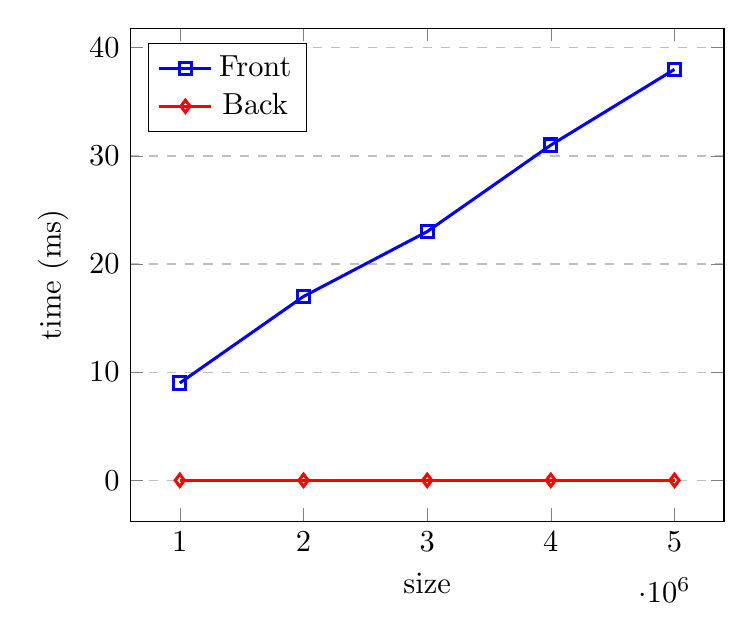
\begin{tikzpicture}[scale=1.1]
			\begin{axis}[
					xlabel={size},
					ylabel={time (ms)},
					ymajorgrids=true,
					grid style=dashed,
					legend pos=north west,
				]
				\addplot[
					color=blue,
					mark=square,
					line width=1pt,
				]
				coordinates {
						(1000000, 9)(2000000, 17)(3000000, 23)(4000000, 31)(5000000, 38)
					};
				\addlegendentry{Front}

				\addplot[color=red,
					mark=diamond,
					line width=1pt,]
				coordinates {
						(1000000, 0)(2000000, 0)(3000000, 0)(4000000, 0)(5000000, 0)
					};
				\addlegendentry{Back}

			\end{axis}
		\end{tikzpicture}
	\end{center}

\end{frame}

\begin{frame}
	\frametitle{Example: Matching Parentheses}
	Here we assume that only parentheses $()$, braces $\{\}$, and brackets $[]$ are allowed.

	Clearly, each opening symbol must match its corresponding closing symbol. For example:
	\begin{itemize}
		\item Correct: $()(())\{([()])\}$
		\item Incorrect: $(\{[])\}$
	\end{itemize}
	The key point: \textbf{the openings are pushed into a stack, and when a closing is encountered, it must match the opening at the top of the stack.}
\end{frame}

\begin{frame}[fragile]
	\begin{minted}[fontsize=\small,breaklines=true,bgcolor=LightGray]{python}
def is_matched(expr):
    openings = '([{'
    closings = ')]}'
    s = Stack()
    for c in expr:
        if c in openings:
            s.push(c)
        elif c in closings:
            if s.is_empty():
                return False
            if TODO:
                return False
    return s.is_empty()
    \end{minted}

\end{frame}

\begin{frame}[fragile]
	\frametitle{1.4 Iterator}
	We would also expect that \alert{Stack} is iterable.
	\begin{columns}
		\column{0.475\textwidth}
		\begin{minted}[bgcolor=LightGray]{python}
a = [1, 9, 4, 6]
for i in a:
    print(i)    
    \end{minted}
		\column{0.475\textwidth}
		\begin{minted}[bgcolor=LightGray]{python}
s = Stack()
s.push(1)
s.push(2)
s.push(3)
for i in s:
    print(i)
    \end{minted}

	\end{columns}
\end{frame}

\begin{frame}[fragile]
	\frametitle{Revisit}
	To make \alert{Array} iterable, we have implemented both \texttt{\_\_len\_\_()} and \texttt{\_\_getitem\_\_()}. What about \alert{Stack}?
\end{frame}

\begin{frame}[fragile]
	Another way to make an ADT iterable is to implement \texttt{\_\_iter\_\_()} which returns an iterator.

	\begin{minted}[bgcolor=LightGray]{python}
def __iter__(self):
    return reversed(self._data)
    \end{minted}

	It is also possible but cumbersome to implement an iterator class manually.
\end{frame}

\begin{frame}[fragile]
	\begin{minted}[fontsize=\small,bgcolor=LightGray]{python}
class ReverseListIterator:
    def __init__(self, data):
        self._data = data
        self._i = len(data)

    def __next__(self):
        if self._i == 0:
            raise StopIteration
        self._i -= 1
        return self._data[self._i]
    \end{minted}

	\begin{minted}[fontsize=\small,bgcolor=LightGray]{python}
def __iter__(self):
    return ReverseListIterator(self._data)        
        \end{minted}
\end{frame}

{\setbeamercolor{palette primary}{fg=black, bg=yellow}
\begin{frame}[standout]
	If you would like a LIFO data structure in Java, never use \href{https://docs.oracle.com/en/java/javase/11/docs/api/java.base/java/util/Stack.html}{java.util.Stack}. You can either use a \href{https://docs.oracle.com/en/java/javase/17/docs/api/java.base/java/util/Deque.html}{java.util.Deque}, or implement it on your own.
\end{frame}
}

\end{document}
